\chapter{Future Work}
\label{Cha:Future_Work}
This chapter list the aspect of Cisco system and Indoor location based service work, for future semesters.

\begin{itemize}
	\item Research better ways of obfuscating the MAC-addresses so it is not stored in plain text.
	\item Secure the connection between Cisco system and the DB server, so data is not possible to sniff.
\end{itemize}


\section{Data Flow from Cisco to the Database}\label{sec:data_flow}
\begin{figure}[ht]
	\begin{center}
		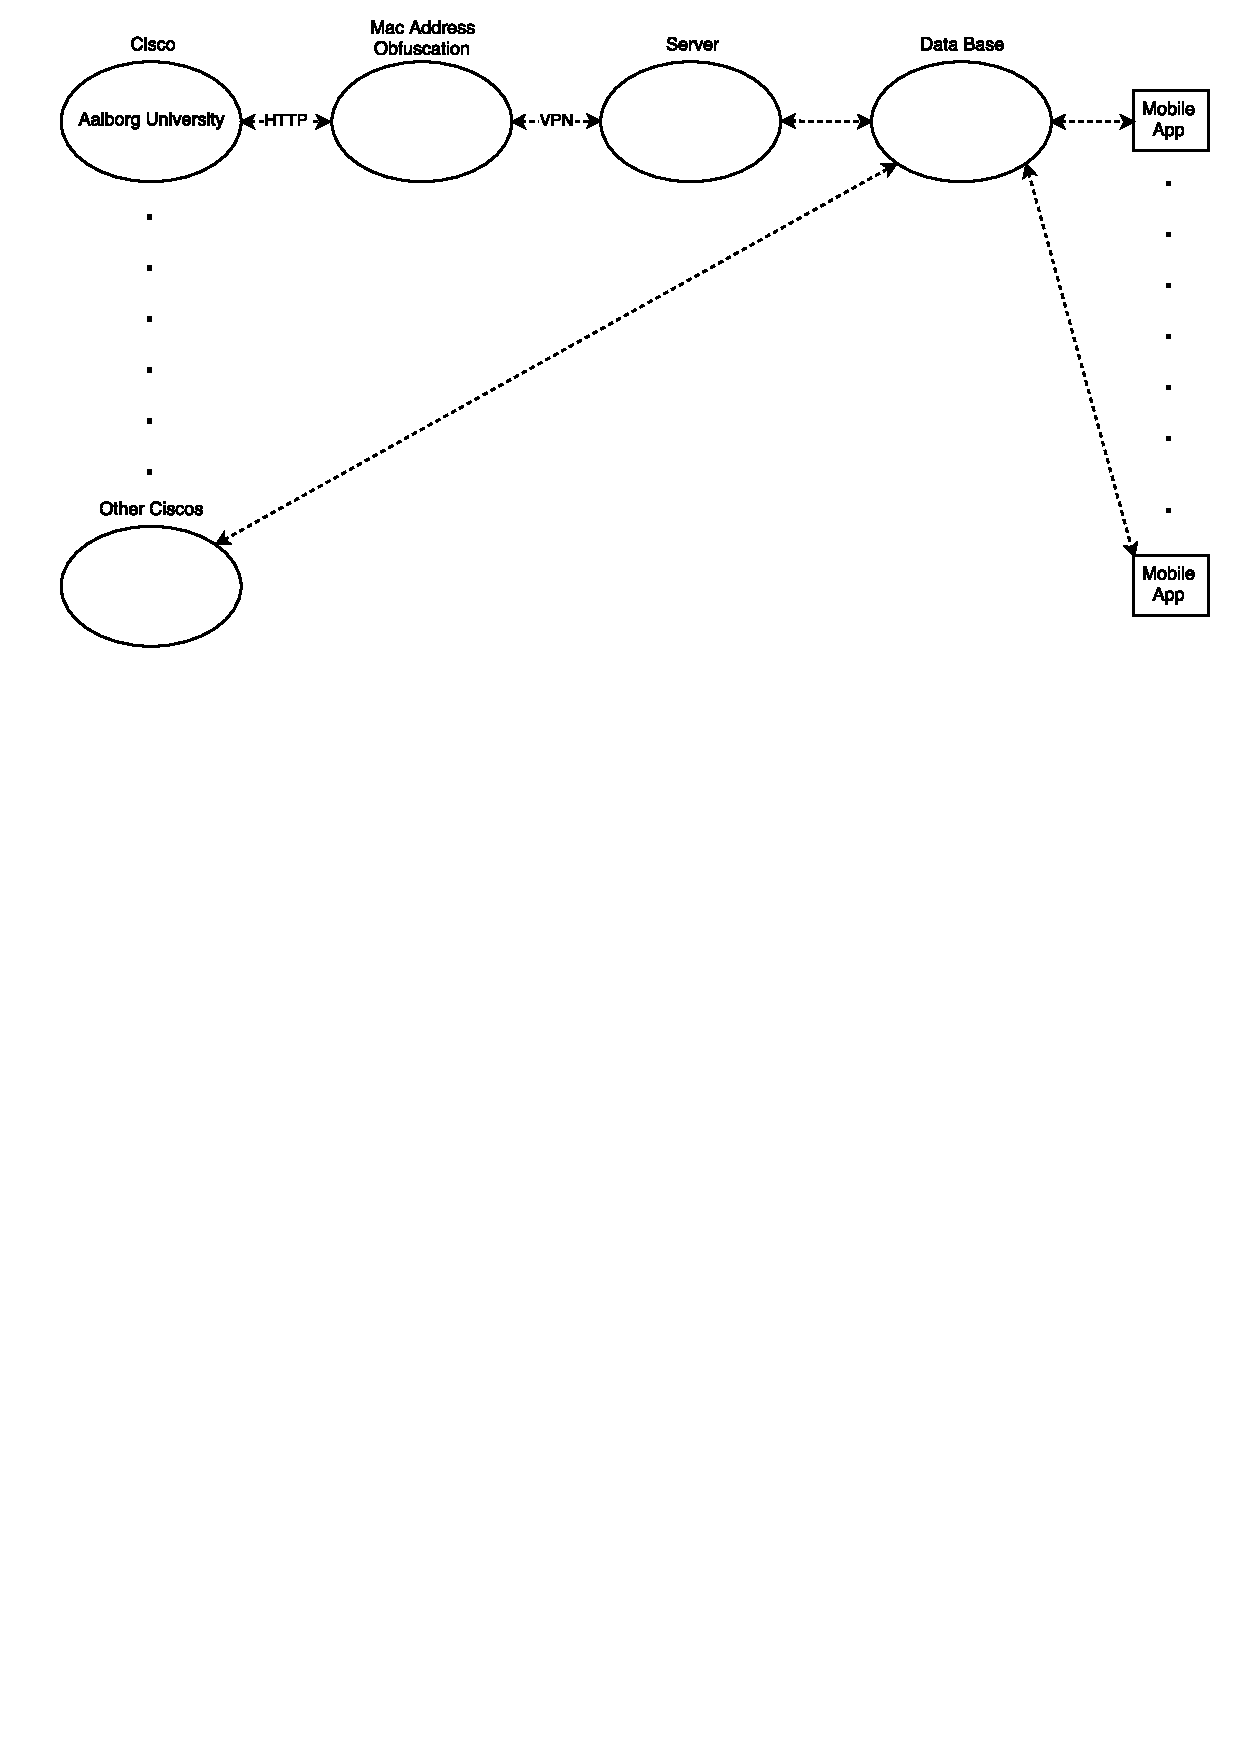
\includegraphics[scale=0.7]{graphics/ciscoSmall.pdf}
		\caption{Cisco systems}
		\label{fig:cisco_systems}
	\end{center} 
\end{figure}
\Cref{fig:cisco_systems} shows how the information flow is intended. The client connecting to the Cisco services can function as a server that requests data from all Cisco services that we have access to. Alternatively, a server can be implemented for each Cisco service. However, this solution has several downsides. First, it means corporations supplying the aStep project with information will have to have hardware running the server, which requires maintenance. Second, this solution is not scalable. The server running the aStep database will potentially be overloaded, as it has to handle each individual Cisco system sending information. As more Cisco systems are added, there will be less time to process received data. An alternative approach is to have the aStep database server request data from the mobile apps, however, with an increase in connected Cisco systems, the interval at which we receive new information from a given system also increases. The optimal solution to this issue is to create a hierarchy of servers, such that the database server only receives data from a constant amount of intermediate servers, each of which also receive information from an amount of sources. During the start up of the aStep project we have access to a single Cisco MSE system, and as such we will not focus on building this hierarchy. However, as the project grows and additional Cisco systems are integrated, it will eventually become a necessity.  